\documentclass[12pt, a4paper, openright]{report}
\usepackage[T1]{fontenc}
\usepackage[utf8]{inputenc}
\usepackage[english]{babel} %Met en français
\usepackage[top=1.5cm, bottom=2.5cm, left=2.5cm, right=2.5cm]{geometry} %changement du cadre
\usepackage{setspace} %Modification des interlignes
\usepackage{graphicx} %insertion d'image
\usepackage{multirow}
\usepackage{booktabs} %Excel2LaTeX
\usepackage{tikz}
\usepackage{amsmath}
\usepackage{amsfonts}
\usepackage{fancyhdr}
\usepackage{lastpage}
\usepackage{lmodern}
\usepackage{mathtools, bm}
\usepackage{amssymb, bm}
\usepackage{libertine}
\usepackage{pdflscape}
\usepackage{wrapfig}
\usepackage{eurosym}
\usepackage{url}
\usepackage{titletoc}
\usepackage[demo]{adjustbox}
\usepackage{xcolor}
\usepackage{tikzpagenodes} 
\usepackage{tabularx,colortbl}              
\usetikzlibrary{calc}        
\usepackage{lipsum}           
\usetikzlibrary{calc}
\usepackage{ifthen}
\usepackage[contents={},opacity=1,scale=1.485]{background}
\definecolor{bleuONE}{RGB}{0,112,192}
\definecolor{vertONE}{RGB}{112, 173, 71}
%%%%%%%%%%%%%%%%%%%%%%%%%%%
% Définition des couleurs %
%%%%%%%%%%%%%%%%%%%%%%%%%%%
\fancypagestyle{pagedegarde}{%
	\fancyhf{}
	\fancyhead[LO]{%
		\begin{tikzpicture}[overlay,remember picture]
		\fill [color=bleuONE] (current page.north west) rectangle
		($ (current page.south west) + (1cm,0cm) $);
		\end{tikzpicture}
	}
	\fancyhead[RE]{%
		\begin{tikzpicture}[overlay,remember picture]
		\fill [color=bleuONE](current page.north east) rectangle
		($ (current page.south east) + (-1cm,0cm) $);
		\end{tikzpicture}
	}
	\fancyfoot[C]{DOCUMENT TITLE - Ref : [REF]} % Footer à modifier ici
	\renewcommand{\headrulewidth}{0pt}
	\renewcommand{\footrulewidth}{0pt}
}
\fancypagestyle{changelog}{%
	\fancyhf{}
	\fancyhead[LO]{%
		\begin{tikzpicture}[overlay,remember picture]
		\fill [color=bleuONE] (current page.north west) rectangle
		($ (current page.south west) + (1cm,0cm) $);
		\end{tikzpicture}
	}
	\fancyhead[RE]{%
		\begin{tikzpicture}[overlay,remember picture]
		\fill [color=bleuONE](current page.north east) rectangle
		($ (current page.south east) + (-1cm,0cm) $);
		\end{tikzpicture}
	}
	\fancyfoot[C]{Ref : [REF]} % Footer à modifier ici

	\renewcommand{\headrulewidth}{0pt}
	\renewcommand{\footrulewidth}{0pt}
}
\fancypagestyle{plain}{%
	\fancyhf{}
	\fancyhead[LO]{%
		\begin{tikzpicture}[overlay,remember picture]
		\fill [color=bleuONE] (current page.north west) rectangle
		($ (current page.south west) + (1cm,0cm) $);
		\end{tikzpicture}
	}
	\fancyhead[RE]{%
		\begin{tikzpicture}[overlay,remember picture]
		\fill [color=bleuONE](current page.north east) rectangle
		($ (current page.south east) + (-1cm,0cm) $);
		\end{tikzpicture}
	}
	\cfoot[C]{Ref : [REF]} % Footer à modifier ici
	\rhead{\begin{picture}(0,30) \put(0,0){
\includegraphics[width=2cm]{logooneblack}} \end{picture}}
	\rfoot{Page \thepage}

}

\begin{document}
		%%%%%%%%%%%%%%%%%
		% Page de garde %
		%%%%%%%%%%%%%%%%%
	
		\pagestyle{pagedegarde}
		\sffamily
		%%%%%%%%%%%%%%%%%%%%%%%%%%%%%%%
		% Titre/Langue/Logo/Codebarre %
		%%%%%%%%%%%%%%%%%%%%%%%%%%%%%%%
		\hfill
\includegraphics[height=2.5cm]{logooneblack}\\
		\noindent\textbf{\textcolor{orange}{[DOCUMENT TYPE] – IPSA ONE 2019}}\hfill
		
\includegraphics[height=1.5cm]{codebarre}\\
		\textbf{\textcolor{vertONE}{ENGLISH}} \\
		
		\vspace*{5pt}
		

		
		\begin{center}
			%%%%%%%%%%%%%%%%%%%%%%%%%%%%
			% Image + cartouche du doc %
			%%%%%%%%%%%%%%%%%%%%%%%%%%%%
			\framebox(479,85){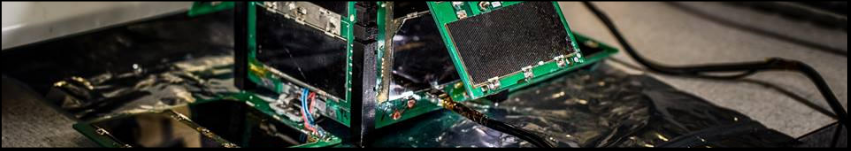
\includegraphics[height=85pt]{image1}}\\
			\vspace{0.3cm}
			%%%%%%%%%%%%%%%%%
			% Cartouche doc %
			%%%%%%%%%%%%%%%%%
			
			\framebox(479,85){ \hfill\begin{minipage}[]{16.5cm}
					\hfill\textbf{TITLE OF THE MISSION}
					\hfill\flushright\large\textbf{\textcolor{bleuONE}{DOCUMENT TITLE}}
					\flushright \normalsize \textbf{\hfill \textcolor{gray}{[MONTH] [YEAR]}}
				\end{minipage} }
		\end{center}
		%%%%%%%%%%%%%%%%%%%%%%
		% Tableau Written by %
		%%%%%%%%%%%%%%%%%%%%%%
		\framebox(238,85){\begin{minipage}[]{10cm}
				\begin{center}
					Written by :\\
					Lucas Bellegy\\
					\vspace{0.5cm}
					
				\end{center}
				
				
				
		\end{minipage}}
	%%%%%%%%%%%%%%%%%%%%%%%%%%
	% Tableau Date signature %
	%%%%%%%%%%%%%%%%%%%%%%%%%%
	\framebox(238,85){\begin{minipage}[]{10cm}
			\begin{center}
				Date and signature :\\
				\vspace{1cm}
			
			
		\end{center}
			
	\end{minipage}}
\noindent
	%%%%%%%%%%%%%%%%%%%%%%
	% Tableau Checked by %
	%%%%%%%%%%%%%%%%%%%%%%
	\framebox(238,85){\begin{minipage}[]{10cm}
			\begin{center}
				Checked  by :\\
				\vspace{0.5cm}
				
			\end{center}
			
			
			
	\end{minipage}}
	%%%%%%%%%%%%%%%%%%%%%%%%%%
	% Tableau Date signature %
	%%%%%%%%%%%%%%%%%%%%%%%%%%
	\framebox(238,85){\begin{minipage}[]{10cm}
			\begin{center}
				Date and signature :\\
				\vspace{1cm}
				
				
			\end{center}
			
	\end{minipage}}
\vspace{3pt}
%%%%%%%%%%%%%%%%%
% ZONE DE LOGOS %
%%%%%%%%%%%%%%%%%
\begin{center}
	
\includegraphics[height=2.15cm]{ipsa} \qquad
	
\includegraphics[height=2.15cm]{logooneblack}\qquad
	
\includegraphics[height=2.15cm]{logoionis}\\
	
\includegraphics[height=2.15cm]{sodern}\qquad
	
\includegraphics[height=2.15cm]{icare}
\end{center}
		%%%%%%%%%%%%%%%%%%%%%%%%
		% Footer page de garde %
		%%%%%%%%%%%%%%%%%%%%%%%%
		\begin{center}
			\footnotesize
			\textbf{O}rbital \textbf{N}ano \textbf{E}xperiments\\
			Association Law 1901 hosted at Institut Polytechnique des Sciences Avancées\\
			63 boulevard de Brandebourg – 94200 Ivry-Sur-Seine\\
			Mail : ipsa-one@ipsa.fr
		\end{center}
	\newpage
	%%%%%%%%%%%%%%%%%%%
	% Page change log %
	%%%%%%%%%%%%%%%%%%%
	\pagestyle{changelog}   % activate colored margins
	\hfill
\includegraphics[height=2cm]{logooneblack}
	\begin{center}
		\textbf{\Large CHANGE LOG}
		\vspace{1cm}
		
		\begin{tabular}{|c|c|c|c|}
			\hline
			\rowcolor{lightgray}
			Ed. & Rev. & Date & Modifications\\
			\hline
			1 & 0 & 13/04/2020 & \qquad \qquad \qquad Document creation \qquad \qquad \qquad \qquad\\
			\hline  
			&  & & \\ 
			\hline    
			&  & & \\ 
			\hline
			&  & & \\ 
			\hline
			&  & & \\ 
			\hline
			&  & & \\ 
			\hline
			&  & & \\ 
			\hline   
		\end{tabular}
	\end{center}
	\tableofcontents % table des matières
	\newpage
    
    
    
    
	
   \section{Les types de liaisons}
\subsection{UART}
La liaison UART, ou liaison série, est une liaison dite asynchrone avec laquelle seulement 2 éléments peuvent communiquer entre eux. C’est-à-dire qu’il n’y a pas d’horloge qui définit la fréquence à laquelle sont envoyées les données. Il y a 2 broches, RX et TX, l’une est pour la réception d’information et l’autre pour l’envoi d’information. Comme il n’y a pas d’horloge pour définir la fréquence de transmission, on doit, pour tout échange de données, paramétrer un nombre de baud(bits/sec).
\subsection{I2C}
La liaison I2C est une liaison synchrone qui permet la communication de théoriquement autant d’appareils qu’on veut. En réalité, une adresse est implémentée dans chaque élément communiquant sur la liaison I2C et ensuite le maître (Master) choisira l’adresse du composant esclave (Slave) avec lequel il veut communiquer. La communication en I2C se fait sur 2 broches, SCL, l’horloge et SDA, la où les données sont échangées.

\section{Les Processeurs}
\subsection{Architecture d’un processeur}
Un processeur est un regroupement de beaucoup de transistors (vraiment beaucoup) qui permettent de créer des portes logiques pour ensuite effectuer différentes actions. Ces actions vont pouvoir être exécutées un certain nombre de fois dans une seconde, c’est ce qu’on appelle la fréquence du processeur. Associé à ces transistors, il y a de la RAM (Random Access Memory) qui permet pendant l’exécution d’un programme l’enregistrement de plusieurs donnée nécessaires à la suite de l’exécution du programme. La RAM s’efface à chaque fois que le processeur est éteint. Il y a aussi la ROM (Read Only Memory), une mémoire qui ne s’efface pas et sur laquelle sont enregistrées les différentes instructions pour l’exécution du programme.
\subsection{Les différents processeurs}
La carte ARM mbed LPC1768 est une carte programmable de petite taille et qui consomme peu, ce qui permet donc d’être très facilement intégrée à un système embarqué. Elle possède 25 broches programmable plus les broches d’alimentions.
L’autre processeur sur lequel nous avons travaillé est le SAMV71Q21 d’Atmel. Cette carte est plus développée que celle de mbed, elle dispose de nombreux ports, capteurs et types de mémoires différents pour faire des tests. On a accès à des  Il est conseillé d’utiliser des gants pour la manipuler. 
Nous avons aussi différents capteurs (la plupart fonctionnant en UART) que nous pouvons utiliser pour faire des programmes tests.
\subsection{Le mapping}
Un mapping de la ARM mbed LPC1768 et les différents capteurs est en cours mais pas encore fini.
\subsection{Les environnements de développement}
L’environnement de développement sur mbed se fait entièrement en ligne et le développement se fait en c++ avec les bibliothèques développées par mbed. Cependant, cet environnement de développement ne nous laisse pas une entière liberté pour regarder dans les bibliothèques ou voir les erreurs exactes. Heureusement il est aussi possible de développer avec visual code ce qui permet de régler les problèmes précédemment cités.
Pour le MCU SAMV71, on doit utiliser le logiciel Atmel Studio. L’initialisation des différentes bibliothèques (composants, horloges, fonctions, variables) disponibles est faite automatiquement, ce qui permet de simplement écrire son code dans un fichier « main.c » (le langage est soit le C soit le C++). On peut aussi utiliser le site Atmel Start pour générer des codes spécifiques avec les bibliothèques des différents capteurs et autres drivers. On a aussi accès à des codes exemples. 

\section{Programmation}
\subsection{Principe}
Une machine ne communique à la base qu’en binaire et ce serait une tache infiniment compliquée que d’écrire des programmes aussi complexes qu’aujourd’hui en binaire. C’est pour ça qu’on utilise des langages de programmation. Ainsi, on peut programmer des taches avec un langage qui nous est bien plus facile à comprendre et ce code sera ensuite compilé pour qu’il puisse être compris par la machine.
\subsection{Compilateur}
Un compilateur est un programme qui va prendre en entrée un code source écrit dans le langage informatique de notre choix, ici, le c++, et va le transformer en un langage objet, un langage exécutable par la machine. Pour faire ceci, Le compilateur va découper le code en ce qu’on appelle des tokens puis, il va analyser ces tokens pour identifier la structure syntaxique du programme (comment il est écrit, y-a-t-il des erreurs dans l’écriture), il va ensuite vérifier s’il n’y a pas d’autre type d’erreur comme la mauvaise déclaration d’une variable ou d’une fonction, il va ensuite générer un code intermédiaire pour appliquer des optimisations et enfin créer le code objet final.
\subsection{Programmation de la communication avec l’antenne}
L’antenne fonctionne exactement comme une simple liaison UART, il suffit donc d’utiliser la bibliothèque mbed pour utiliser la liaison UART.

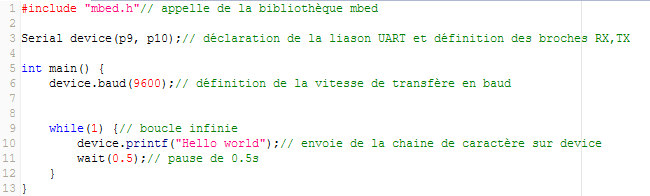
\includegraphics[]{aaa.png}



\section{Feedback sur la phase I}
- Récupérer le plus de documents possibles
- Ajouter la liaison CAN à la documentation
- Faire des recherches supplémentaires sur le fonctionnement de la mémoire, les périphériques, la DMA, MMU
- Créer des tutos pour l'utilisation des logiciels (Atmel Studio)
	
	\clearpage
	\pagestyle{plain}    % Revenir sur le style sans margin
	
	
	
	
\end{document}